\def\VCDate{2016/03/15}\def\VCVersion{(Current)}
\documentclass{article}
\usepackage[screen]{geometry}
\usepackage[hypcap]{caption}
\usepackage{ProofPower, verbatim, graphicx, color, amsmath, amssymb, hyperref, multicol}
\begin{document}
\underscoreoff

\title{CS118 Lab:1}
\author{Saw Thinkar Nay Htoo}
\maketitle

\section*{}
\# \href{http://keepachangelog.com}{Change Log} \\
All changes to this lab will be documented in this section. 
\bigskip \\
\#\# [0.3.0] - 2016-03-04 \\
\#\#\# Added \\
- \hyperlink{1}{Detailed explanation of the algorithm.} \\
- \hyperlink{2}{Detailed explanation of the SML code.} \\
- \hyperlink{3}{Detailed explanation of the C code.} \\
- \hyperlink{4}{Detailed explanation of the ASM code.} 
\bigskip \\
\#\#\# Changed \\
- labasm file was not compiled due to the usage of \hyperlink{5}{"add"} error. Now corrected to \verb|add %eax,%ebx.| 
\bigskip \\
\#\# [0.3.0] - 2016-03-08 \\
\#\#\# Added \\
- \hyperlink{6}{C to ASM translation of code to illustrate the concept} \\
- \hyperlink{7}{3 functions called}
\clearpage

\section*{Choosing a car}
An algorithm is described to help select the best car based on overall cost related to fuel efficiency.
\begin{description}
\item[Inputs] : purchase price (in \$)and fuel efficiency (in mpg)
\item[Process] :\\
anuual fuel cost = price per gallon times the annual fuel consumed \\
operating cost = years times annual fuel cost \\
total cost = purchase price + operating cost \\
\item[Output] : total cost
\end{description}

\clearpage

\section*{Analysis}
Assume the number of years to use this car be 10. \\
And let the milage of the car be 15,000 miles per year and gas cost be \$3 per gallon. \\
Purchase price of car is \$25,000 and fuel efficiency is 45 miles per gallon. \\
So by using above information, the total cost is calculated which is the sum of the purchase price and operating cost of the car. 
\footnote{This is the algorithm to formulate the calculation of the total cost.}
 
\begin{description}
\item[\hypertarget{1}{Detailed explanation of the algorithm to calculate the total cost.}]
\item[Inputs:] : purchase price (in \$) and fuel efficiency (in mpg)
\item[Process:] :\\
annual fuel cost = 3 times 15000/45 \\
In the above equation, 15,000 miles per year is divided by 45 miles per gallon to give the result of annual fuel usage of 333.33 gallons per year. The annual fuel usage is multiplied with \$3 per gallon to give the result of annual fuel cost which is \$1000. \\
operating cost = 10 times annual fuel cost \\
In the above equation, annual fuel cost of \$1000 times 10 years gives the results of the operating cost of \$10,000 of the car for 10 years. \\
total cost = 25000 + operating cost \\
In the above equation, the calculated operating cost is added with purchasing price of the car which is \$25,000 to give the final result of the total cost; \$35,000. 
\item[Output:] total cost
\end{description}
\clearpage

\section*{SML code for the algorithm} 
\hypertarget{2}{Detailed explanation of the SML code.} \\
In this section, I try to break down the SML code into several steps making the algorithm as simple as possible for further coding with different programming languages. 
\begin{GFT}{SML}
\+fun annual\_fuel\_consumed(ppg,mpy,mpg) = ppg*mpy div mpg;\\
\+val ppg = 3; val mpy = 15000; val mpg = 45;\\
\+val fuel = annual\_fuel\_consumed(ppg,mpy,mpg);\\
\end{GFT}
-Function "annual_fuel_consumed" is created with three parameters which are ppg, price per gallon; mpy, miles per year; and mpg, miles per gallon. \\
-Variables ppg, mpy and mpg are declared as 3, 15000 and 45 respectively. \\
-The result function "annual_fuel_consumed" assigned to variable "fuel", which is 1000. \\
-Below is the output of the above SML code. \\
\smallskip \\
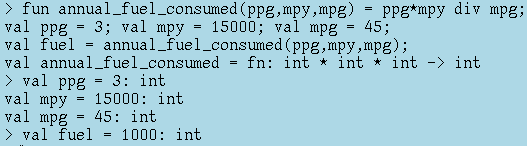
\includegraphics[scale =0.6]{fuelsml.png} \\
\noindent{\color{red}\rule{\linewidth}{0.5mm}}
\clearpage 

\begin{GFT}{SML}
\+val years = 10; \\
\+fun operating\_cost(fc) = years * fc;\\
\+val cost = operating\_cost(fuel);\\
\end{GFT}
-Variable "years" is assigned as 10. \\
-Function "operating_cost" is created. \\
-Function "operating_cost" is operated using the parameter "fuel", which is calculated previously. Then the result of the function is assigned to the variable "cost" which is 10000. \\
-Below is the output of the above SML code. \\
\smallskip \\
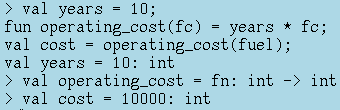
\includegraphics[scale =0.6]{costsml.png} \\
\noindent{\color{red}\rule{\linewidth}{0.5mm}}
\begin{GFT}{SML}
\+val pp = 25000; \\
\+fun total\_cost(oc) = pp + oc;\\
\+val total = total\_cost(cost);\\
\end{GFT}
-Variable "pp" is assigned as 25000. \\
-Function "total_cost" is created. \\
-The function is operated using the parameter "cost", which is calculated previously. Then the result of the function is assigned to the variable "total", which is the final result, 35000. \\
\clearpage

-Below is the output of the above SML code. \\
\smallskip \\
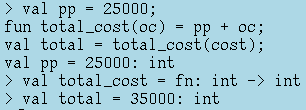
\includegraphics[scale =0.6]{totalsml.png} \\
\noindent{\color{red}\rule{\linewidth}{0.5mm}} 
\section*{Overall output from SML code}
\verbatiminput{result.out}
\verbatiminput{cresult}
\clearpage

\section*{C code implementation of the SML code}
\hypertarget{3}{Detailed explanation of the C code.} \\
-Global variables are declared which can be accessed by functions starting from third line of following code. 
\begin{GFT}{Text written to file lab1.c}
\+\#include <stdio.h>\\
\+int eax; int ebx; int ecx;\\
\+int fuel; int cost; int total;\\
\end{GFT}
\noindent{\color{red}\rule{\linewidth}{0.5mm}}
-annual_fuel_consumed2 function, operating_cost2 function and total_cost2 function are declared. Variables "years" and "pp",(purchasing price), are defined as 10 and 25000 respectively.
\begin{GFT}{Text appended to file lab1.c}
\+//int annual\_fuel\_consumed(int ppg,int mpy,int mpg)\\
\+//\{return ppg* mpy/mpg;\}\\
\+int annual\_fuel\_consumed2()\{return eax = eax * ebx / ecx;\}\\
\+\#define years 10\\
\+//int operating\_cost(int fc) \{return years * fc;\}\\
\+void operating\_cost2()\{eax = years * eax;\}\\
\+\#define pp 25000\\
\+//int total\_cost(int msgoc)\{return pp + oc;\}\\
\+int total\_cost2()\{return pp + eax;\}\\
\end{GFT}
\noindent{\color{red}\rule{\linewidth}{0.5mm}} \\
\clearpage

-Variables "ppg", "mpy" and "mpg" are defined as 3, 15000 and 45 respectively.
\begin{GFT}{Text appended to file lab1.c}
\+\#define ppg 3\\
\+\#define mpy 15000\\
\+\#define mpg 45\\
\end{GFT}
\noindent{\color{red}\rule{\linewidth}{0.5mm}}
-eax, ebx and ecx are assigned with each variable mentioned in above code. \\
\begin{multicols}{2}
\begin{GFT}{Text appended to file lab1.c}
\+int main()\\
\+\{\\
\+eax = ppg;\\
\+ebx = mpy;\\
\+ecx = mpg;\\
\end{GFT}
\columnbreak
\centering
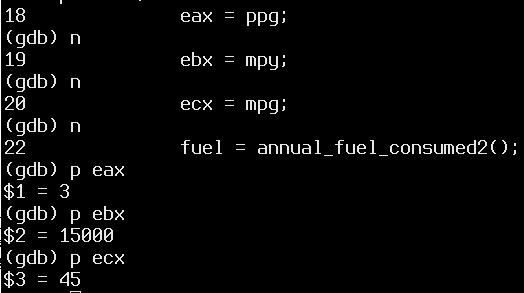
\includegraphics[scale = 0.4]{varc.png}
\end{multicols}
\noindent{\color{red}\rule{\linewidth}{0.5mm}} \\

\clearpage

-In this case, since this C code is written in the most similar syntax of ASM code, it is assumed that most recently returned value is assigned to eax. \\
-After the result of the variable "fuel" is produced using function "annual_fuel_consumed2", its value of 1000 is assigned to "eax".
\begin{multicols}{2}
\begin{GFT}{Text appended to file lab1.c}
\+//fuel = annual\_fuel\_consumed(ppg,mpy,mpg);\\
\+fuel = annual\_fuel\_consumed2();\\
\+eax = fuel;\\
\end{GFT}
\columnbreak
\raggedleft
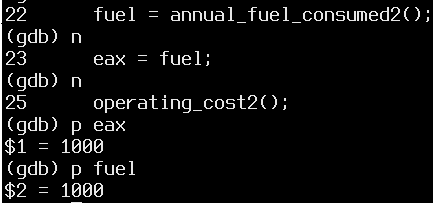
\includegraphics[scale=0.4]{afcc.png}
\end{multicols}
\noindent{\color{red}\rule{\linewidth}{0.5mm}} \\

-According to the function, "operating_cost2", declared in the global, the result of the above function, "annual_fuel_consumed2", which is assigned to eax will be times with years of 10, producing the output of 10000. 
\begin{multicols}{2}
\begin{GFT}{Text appended to file lab1.c}
\+//cost = operating\_cost();\\
\+operating\_cost2(); \\
\+//assume return value is in eax\\
\+//cost = eax;\\
\end{GFT}
\columnbreak
\raggedleft
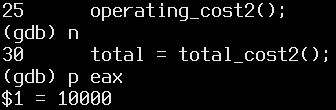
\includegraphics[scale=0.5]{occ.png}
\end{multicols}
\noindent{\color{red}\rule{\linewidth}{0.5mm}} \\
\clearpage

-Now as we can see the result of eax, 10000 which is calculated previously, will be added to the "pp",(purchase price of 25000 of the car), through the function "total_cost2", consequently giving out the final result of "total" as 35000. Then the result of "total" is printed out after being assigned to the function "total_cost2", followed by "return" function.
\begin{multicols}{2}
\begin{GFT}{Text appended to file lab1.c}
\+//total = total\_cost(cost);\\
\+//eax = cost;\\
\+total = total\_cost2();\\
\+printf("Total cost of car: \%i\Backslash{}n",total);\\
\+return 0;\\
\+\}\\
\end{GFT}
\columnbreak
\raggedleft
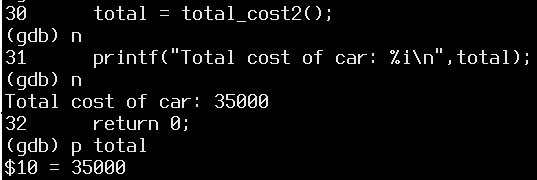
\includegraphics[scale=0.4]{tcc.png}
\end{multicols}
\textbf{\underline{Above C output results on the right columns are operated using \href{https://en.wikipedia.org/wiki/GNU_Debugger}{GDB},the standard }} \\
\textbf{\underline{debugger for the GNU operating system.}} \\
\noindent{\color{red}\rule{\linewidth}{0.5mm}} \\

The output when running the C program in the \href{https://en.wikipedia.org/wiki/Data_Display_Debugger}{data display debugger}, using "ddd" command, is: 

\begin{center}
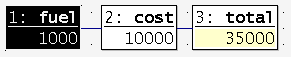
\includegraphics{out1.png}
\end{center}

\clearpage
\section*{Translation of C code to ASM code}
\hypertarget{6}{C to ASM translation of code to illustrate the concept}
\begin{itemize}
\item 
include statements (libraries like stdio) \\
There is no need to include declarations of functions like we need to do in C++ \\
Checklist to skim through. \\
\href{http://goo.gl/UTS9OT}{Assembly Language Library by David Parket} \\
\href{http://goo.gl/EenLOf}{The university of California Riverside Standard Library for 80x86 assembly language}
\item declare variables \\
C code, \verb|"int fuel= 0; int cost= 0; int total = 0;"| is translated into ASM as below. 
\begin{verbatim}
.data
  fuel: .long 0
  total: .long 0
  cost: .long 0
\end{verbatim}
\item 
define functions \\
C code, \verb|"void operating_cost2(){eax = years * eax;}"| is translated as below. 
\begin{verbatim}  
  operating_cost:
  #now eax is 1000
  mov $10, %ebx
  mul %ebx 
  # eax is 10000
  ret
\end{verbatim}
\item 
symbolic constants (in C define) \\
e.g. \verb|#define x 0| in C would be \verb|.equ x,0| in asm
\begin{verbatim}  
  .equ ppg,3 \\
  .equ mpy,15000 \\
  .equ mpg,45 \\
\end{verbatim}
\item 
assignment statements\\
\verb| MOV| \\
\verb|mov $10, %ebx| \\
See \href{http://goo.gl/z4R9io}{IA32 Cheat Sheet}: Left column.
\item 
call assembly language functions
\begin{verbatim}  
 call annual_fuel_consumed
 call operating_cost
 call total_cost
\end{verbatim}
\item 
call C functions (printf) \\
e.g. the call to printf: printf("Total cost of car: \verb|%i\n|",total); in asm is:
\begin{verbatim}  
  push %eax
  push $msg
  call printf
  add $8,%esp
\end{verbatim}
\item 
return from main function 
\begin{verbatim}  
main:
 call annual_fuel_consumed 
 call operating_cost 
 call total_cost 
 ret \\
\end{verbatim}
\item
arithmetic operations (addition, multiplication, integer division) \\
Addition. \\
For addition, the value is moved to the register ebx, then the value of ebx is added to eax. C code: \verb|int total_cost2(){return pp + eax;}|
\begin{verbatim}
  mov $25000, %ebx
  add %ebx,%eax 
\end{verbatim}
Multiplication. \\
For multiplication, two value of numbers are assigned to each register then those two registers are operated using "mul" mnemonic. C code: \verb|int annual_fuel_consumed2(){return eax = eax * ebx / ecx;}|
\begin{verbatim}
  .equ ppg,3 
  .equ mpy,15000  
  mov $ppg,%eax 
  mov $mpy,%ebx 
  mul %ebx 
\end{verbatim}
Integer division. \\
For division, the same procedure is used. Move the value to the register then register is operated by operation instruction "div". C code: \verb|int annual_fuel_consumed2(){return eax = eax * ebx / ecx;}|
\begin{verbatim}
  .equ mpr,45
  mov $mpg, %ecx
  div %ecx 
\end{verbatim}
\end{itemize}
\clearpage

\hypertarget{4}{Detailed explanation of the ASM code.} \\

\begin{GFT}{Text written to file lab1.s}
\+.equ ppg,3 \\
\+.equ mpy,15000\\
\+.equ mpg,45\\
\+.data\\
\+  fuel: .long 0\\
\+  total: .long 0\\
\+  cost: .long 0\\
\+msg: .string "Total cost: \%i\Backslash{}n"\\
\end{GFT}
\verb|.equ ppg,3|  in asm is the same as \verb|#define ppg 3| in C code. As we can see, "ppg", "mpy" and "mpg" are assigned with each value. Section \href{http://goo.gl/4czLEp}{.data} is used to declare initialized data or constants. Unfortunately, I am not sure why these three variables, fuel, total and cost are declared. "msg: .string" works as "printf". \\
\noindent{\color{red}\rule{\linewidth}{0.5mm}} \\

\begin{multicols}{2}
\begin{GFT}{Text appended to file lab1.s}
\+.text\\
\+  annual\_fuel\_consumed:\\
\+  mov \$ppg,\%eax \\
\+  mov \$mpy,\%ebx \\
\+  mul \%ebx \\
\+  \# edx:eax = eax * ebx\\
\end{GFT}
\columnbreak
\raggedleft
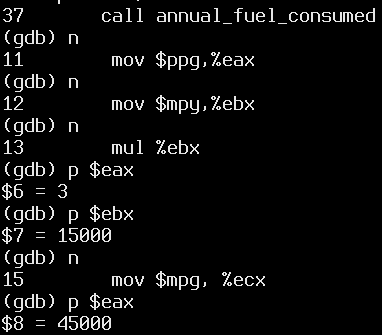
\includegraphics[scale=0.4]{afc1asm.png}
\end{multicols}
Section \href{http://goo.gl/4czLEp}{.text} contains the actual machine instructions. In above function, eax and ebx are \href{http://whatis.techtarget.com/definition/register}{registers}. "mov" and "mul" are used to represent low-level machine instruction or operation, also known as \href{https://www.techopedia.com/definition/28287/mnemonic}{mnemonic}.\\
In the above code, values of "ppg" and "mpy" is moved into eax and ebx registers respectively. In this case, due to the fact that eax is a default or initial register, "ebx" is multiplied with "eax" of 15000, and result is replaced in "eax", using "mul" operator. As we can see the result on the right column, before the "mul" instruction, value of "eax" is 3. After the multiplication, "eax" becomes 45000. \\
\noindent{\color{red}\rule{\linewidth}{0.5mm}} \\

\begin{multicols}{2}
\begin{GFT}{Text appended to file lab1.s}
\+  mov \$mpg, \%ecx\\
\+  div \%ecx \\
\+  \# eax = edx:eax / ecx\\
\+  ret\\
\end{GFT}
\columnbreak
\raggedleft
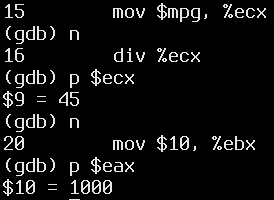
\includegraphics[scale=0.4]{afc2asm.png}
\end{multicols}
Now, "mpg" value of 45 is moved into "ecx". After "eax" is divided by "ecx", a new "eax" result is produced as 1000. \\ 
\noindent{\color{red}\rule{\linewidth}{0.5mm}} \\
\clearpage

\begin{multicols}{2}
\begin{GFT}{Text appended to file lab1.s}
\+  operating\_cost:\\
\+  \#now eax is 1000\\
\+  mov \$10, \%ebx\\
\+  mul \%ebx \\
\+  \# eax is 10000\\
\+  ret\\
\end{GFT}
\columnbreak
\raggedleft
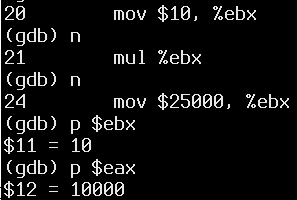
\includegraphics[scale=0.4]{opasm.png}
\end{multicols}
Value 10 is moved into "ebx". Then "ebx" is multiplied with "eax", giving out the 10000. \\
\noindent{\color{red}\rule{\linewidth}{0.5mm}} \\

\begin{multicols}{2}
\begin{GFT}{Text appended to file lab1.s}
\+  total\_cost:\\
\+  mov \$25000, \%ebx\\
\+  add \%ebx,\%eax \\
\+  \# eax is 35000\\
\+  ret\\
\end{GFT}
\columnbreak
\raggedleft
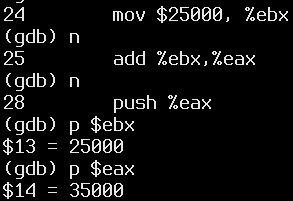
\includegraphics[scale=0.4]{tcasm.png}
\end{multicols}
Then value of 250000 is moved to "ebx", and using \hypertarget{5}{"add"} mnemonic value of "ebx" is added to the value of "eax", which at last results "eax" as 35000. \\
\noindent{\color{red}\rule{\linewidth}{0.5mm}} \\
\clearpage

\begin{multicols}{2}
\hypertarget{7}{3 ASM functions addded.}
\begin{GFT}{Text appended to file lab1.s}
\+  \#below code is to print out\\
\+  push \%eax\\
\+  push \$msg\\
\+  call printf\\
\+  add \$8,\%esp \\
\+  \#below code is for return function\\
\+ ret\\
\+ .globl main\\
\+main:\\
\+ call annual\_fuel\_consumed\\
\+ call operating\_cost\\
\+ call total\_cost\\
\+ ret\\
\end{GFT}
\columnbreak
\raggedleft
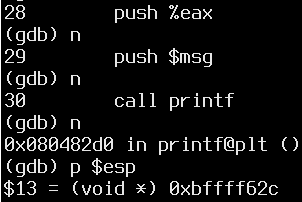
\includegraphics[scale=0.5]{printasm.png}
\end{multicols}
I still need to figure out more with \verb|add $8,%esp| and some of the results above. (I got it during lab2 section: to clean up the stack.)  According to the book, it seems that it is used to clear the pointer register. Basically, "eax" is pushed on the stack. Then the register "esp" is used to point a specific location on the stack to print out the value of "eax". In the final section of the code, function "annual_fuel_consumed" is returned. Below is the final ASM result.\\ 
\bigskip \\
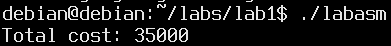
\includegraphics[scale =0.6]{resultasm.png} \\
\noindent{\color{red}\rule{\linewidth}{0.5mm}} \\
\clearpage

\section*{Shell scripts to make processing easier}
This shell script is used to make extracting and processing the source code easier. The -g option to the gcc compiler adds debugging symbols so we can refer to variables even though they are not normally stored in the object code. 

\begin{GFT}{Text written to file labcode.sh}
\+docsml lab1.doc\\
\+gcc -Wall -g -o labc lab1.c\\
\+gcc -Wall -g -o labasm lab1.s\\
\+\\
\end{GFT}
\begin{GFT}{Text written to file labdoc.sh}
\+doctex lab1.doc\\
\+pptexenv /home/debian/texfot.pl pdflatex lab1.tex\\
\+\\
\end{GFT}
\begin{GFT}{Bourne Shell}
\+chmod 755 labcode.sh\\
\+chmod 755 labdoc.sh\\
\+poly < lab1.sml > result.out\\
\+./labc > cresult\\
\+\\
\end{GFT}
\end{document}
